\subsubsection{Scénario Cockburn}
\textbf{Cas d'utilisation:} Sortir

\textbf{Acteur primaire:}  Le conducteur

\textbf{Pré-condition:} La transaction (paiement) a été accepté.

 
\textbf{Post-condition:} Le deuxième barriere est abaissée. 

\textbf{Scenario primaire: } \\
    \textbf{1.}  La borne change la couleur du feu (vert). \\
    \textbf{2.} La borne léve la deuxième barrière. \\
    \textbf{3.} Le conducteur se dirige vers la deuxième barrière.\\
    \textbf{4.} Le deuxième boucle detecte que le véhicule est sorti.\\ 
    \textbf{5.}  La borne change la couleur du feu (rouge).\\
    \textbf{6.}  La borne abaisse la deuxième barrière. \\

\textbf{Variantes:}\\
    \textbf{1a.} Le feu ne change pas de couleur. Donc une alarme est levé vers le technicien. Fin scénario.\\
    \textbf{2a.}  . La deuxième barriere barriere ne se léve pas. Donc une alarme est levé vers le technicien. Fin scenário.\\
    \textbf{4a.}  La boucle ne détecte pas que le véhicule est sortie. La barrière reste levée.Fin scénario.\\
\newpage    
\subsubsection{Diagramme d'activité}
\begin{figure}[!htb]
    \centering
    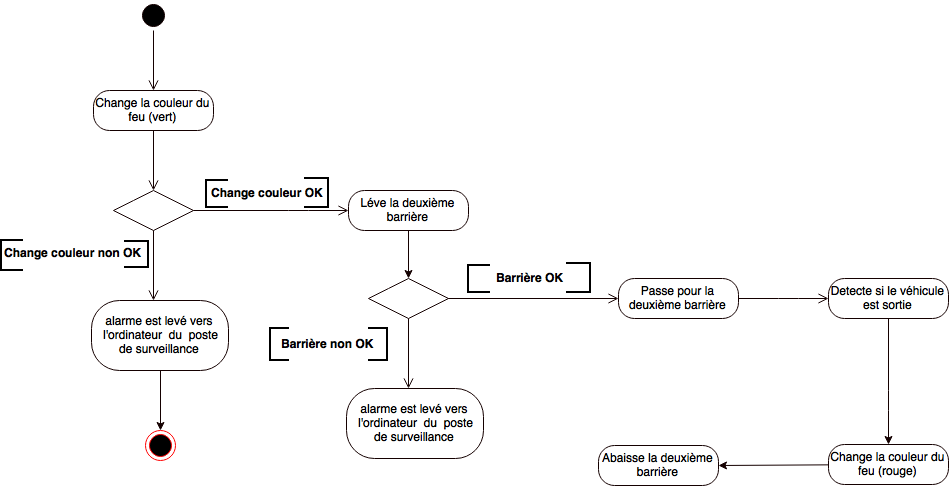
\includegraphics[scale=0.4, angle = 90]{02_Desenvolvimento/TD2/images/DASortir.png}
    \caption{Diagramme d'activité - Sortir}
    \label{fig:DARentrer}
\end{figure}
\newpage    
\subsubsection{Collaboration}
\begin{figure}[!htb]
    \centering
    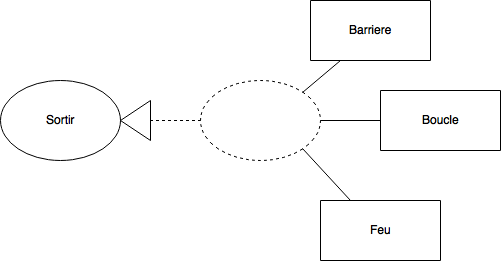
\includegraphics[scale=0.6]{02_Desenvolvimento/TD2/images/ColaSortir.png}
    \caption{Collaboration - Sortir}
    \label{fig:DARentrer}
\end{figure}
\newpage    
\subsubsection{Diagramme de séquence}
\begin{figure}[!htb]
    \centering
    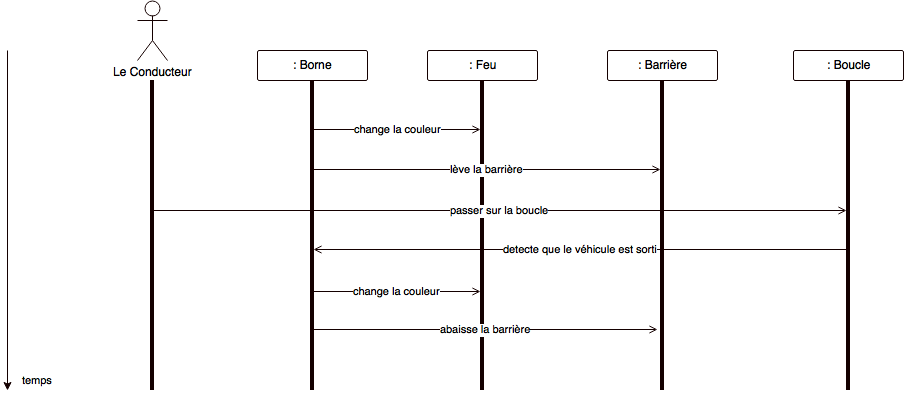
\includegraphics[scale=0.5]{02_Desenvolvimento/TD2/images/DSSortir.png}
    \caption{Diagramme de séquence - Sortir - à revisiter }
    \label{fig:DARentrer}
\end{figure}
\subsubsection{Diagramme de séquence}
\begin{figure}[!htb]
    \centering
    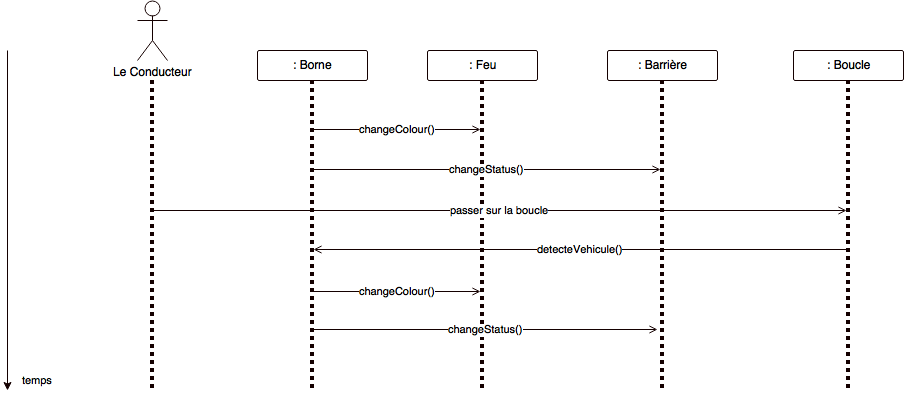
\includegraphics[scale=0.5]{02_Desenvolvimento/TD2/images/v2-DSSortir.png}
    \caption{Diagramme de séquence - Sortir}
    \label{fig:DARentrer}
\end{figure}